% --- Use the 'standalone' class with the 'tikz' option ---
% This creates a document cropped to the size of the drawing
\documentclass[tikz]{standalone}

% --- Load TikZ Libraries ---
% These are required for the matrix, arrows, and positioning
\usepackage{tikz}
\usetikzlibrary{matrix, arrows.meta, positioning}

% --- Color Definitions ---
% We must define the colors here since this is a separate file
% (These should match your main poster's colors)
\definecolor{MyBlue}{RGB}{45, 114, 178}
\definecolor{MyLightBlue}{RGB}{230, 240, 255}

\begin{document}

% --- The TikZ Figure Code ---
% No \begin{figure} is needed, just the drawing itself
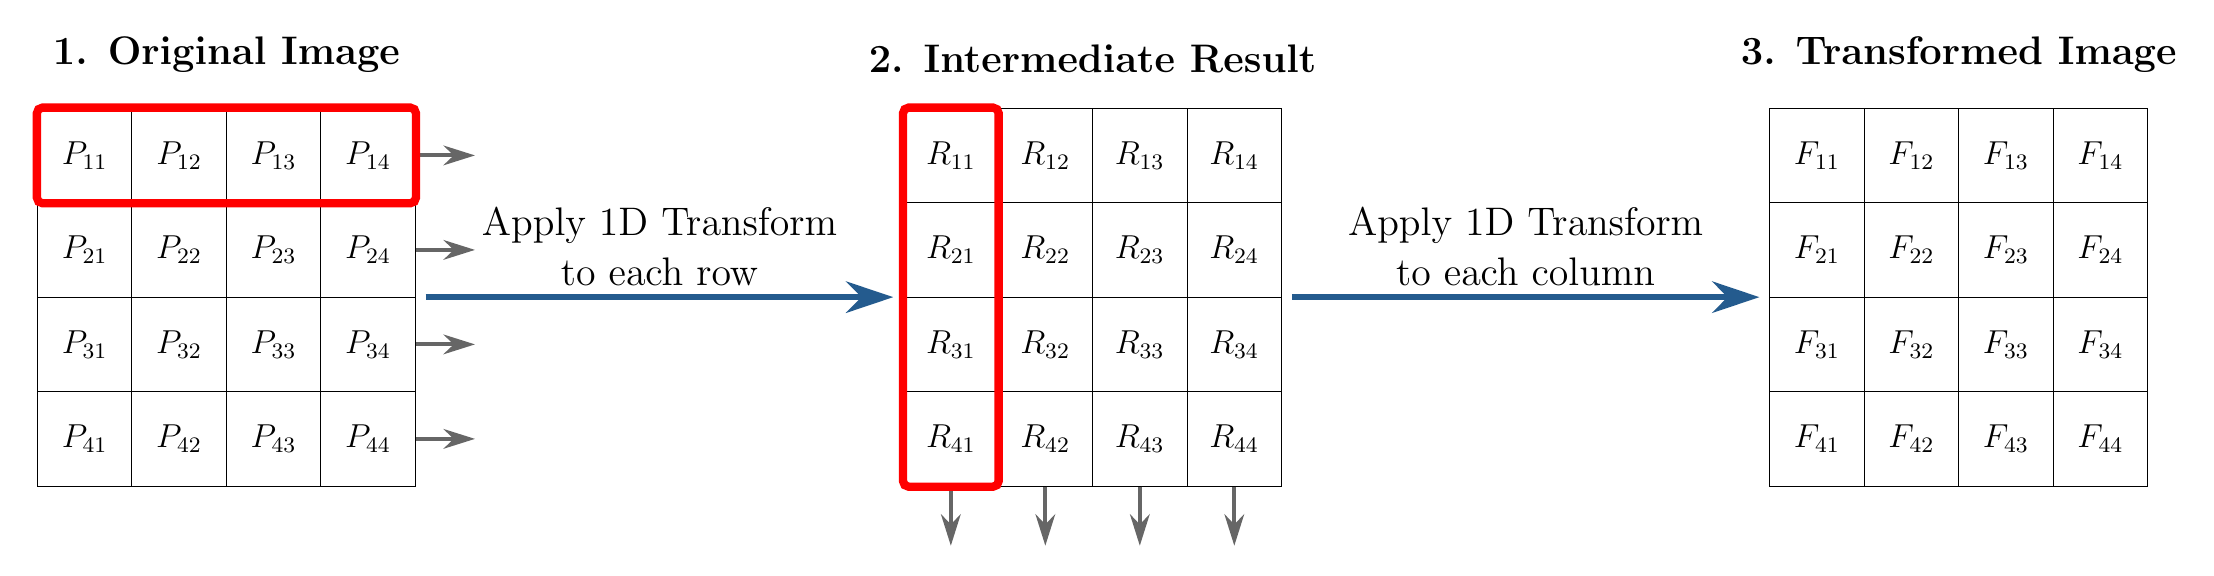
\begin{tikzpicture}[
    % --- Styles ---
    % Style for the 4x4 matrices
    matrix-style/.style={
        matrix of nodes,
        nodes={draw, minimum size=1.2cm, inner sep=0pt, font=\large},
        nodes in empty cells,
        row sep=-\pgflinewidth, % Connect cell borders
        column sep=-\pgflinewidth
    },
    % Style for the big labels on arrows
    arrow-label/.style={
        font=\Large, % Make labels big for poster
        pos=0.5,
        auto,
        align=center % Allow line breaks
    },
    % Style for the big arrows between matrices
    arrow-style/.style={
        -{Stealth[length=6mm, width=4mm]}, % Big arrow heads
        line width=2pt,
        draw=MyBlue!80!black % Use your poster's color
    },
    % Style for the small helper arrows
    small-arrow/.style={
        -{Stealth[length=4mm, width=2.5mm]},
        line width=1.5pt,
        draw=black!60
    }
]

% --- Node 1: Original Image ---
\node[matrix, matrix-style] (img) at (0,0) {
    $P_{11}$ & $P_{12}$ & $P_{13}$ & $P_{14}$ \\
    $P_{21}$ & $P_{22}$ & $P_{23}$ & $P_{24}$ \\
    $P_{31}$ & $P_{32}$ & $P_{33}$ & $P_{34}$ \\
    $P_{41}$ & $P_{42}$ & $P_{43}$ & $P_{44}$ \\
};
\node[above=0.2cm of img, font=\Large\bfseries] (img-label) {1. Original Image};

% --- Small arrows showing row-wise operation ---
\foreach \i in {1,...,4} {
    \draw[small-arrow] (img-\i-4.east) -- ++(0.75,0);
}

% --- Node 2: Intermediate Matrix (Row DFTs) ---
% MODIFIED: Changed x-coordinate from 9 to 11 for more space
\node[matrix, matrix-style] (inter) at (11,0) {
    $R_{11}$ & $R_{12}$ & $R_{13}$ & $R_{14}$ \\
    $R_{21}$ & $R_{22}$ & $R_{23}$ & $R_{24}$ \\
    $R_{31}$ & $R_{32}$ & $R_{33}$ & $R_{34}$ \\
    $R_{41}$ & $R_{42}$ & $R_{43}$ & $R_{44}$ \\
};
\node[above=0.2cm of inter, font=\Large\bfseries] (inter-label) {2. Intermediate Result};

% --- Small arrows showing col-wise operation ---
\foreach \i in {1,...,4} {
    \draw[small-arrow] (inter-4-\i.south) -- ++(0,-0.75);
}

% --- Node 3: Final DFT ---
% MODIFIED: Changed x-coordinate from 18 to 22 for more space
\node[matrix, matrix-style] (final) at (22,0) {
    $F_{11}$ & $F_{12}$ & $F_{13}$ & $F_{14}$ \\
    $F_{21}$ & $F_{22}$ & $F_{23}$ & $F_{24}$ \\
    $F_{31}$ & $F_{32}$ & $F_{33}$ & $F_{34}$ \\
    $F_{41}$ & $F_{42}$ & $F_{43}$ & $F_{44}$ \\
};
\node[above=0.2cm of final, font=\Large\bfseries] (final-label) {3. Transformed Image};

% --- Main Connecting Arrows ---
\draw[arrow-style] (img.east) -- (inter.west) 
    % MODIFIED: Changed **ROW** to row
    node[arrow-label, above] {Apply 1D Transform \\ to each row};

\draw[arrow-style] (inter.east) -- (final.west) 
    % MODIFIED: Changed **COLUMN** to column
    node[arrow-label, above] {Apply 1D Transform \\ to each column};
    
% --- Highlight Example Regions ---
\draw[red, line width=3pt, rounded corners=2pt] 
    (img-1-1.north west) rectangle (img-1-4.south east);
    
\draw[red, line width=3pt, rounded corners=2pt] 
    (inter-1-1.north west) rectangle (inter-4-1.south east);

\end{tikzpicture}

\end{document}